\chapter{其他干预性研究设计}
\chapterauthors{Deborah G. Grady、Steven R. Cummings、Alison J. Huang}
\begingroup\setlength{\tabcolsep}{4pt}
\sourcepage{377}
上一章讨论了经典的个体水平随机、盲法、平行组临床试验。还有其他一些设计，研究者同样实施干预，但改变或省去了经典随机试验的某些方面。本章介绍常用的其他干预性研究设计，以及在适当条件下具有特殊优势的设计。

\section{其他随机设计}
\subsection{析因设计}
\term{析因试验}（factorial trial）旨在一项研究中回答两个或更多不同的研究问题（图12.1）。例如，VITAL试验旨在检验维生素D3和omega-3脂肪酸补充剂对心血管事件与癌症风险的作用。参与者随机分为四组，以检验四个假设。研究结束时，先比较接受维生素D3者与接受相应安慰剂者的心血管事件和癌症发生率，不考虑这两组中各有一半参与者同时接受omega-3脂肪酸；再比较接受omega-3脂肪酸者与接受相应安慰剂者的心血管事件和癌症发生率，同样不考虑每组各有一半人同时接受维生素D3。研究者以一项试验的投入，研究了两项干预和两个结局。遗憾的是，两项干预均未显示益处（1、2）。
% Original PDF pages 378, 381, 385, 388, 391, 394, 397, and 406.
% The original data curves and patient icons are retained where used;
% Chinese labels are overlaid by TeX without changing the source assets.
\definecolor{chTwelveBand}{RGB}{185,204,234}
\definecolor{chTwelveCream}{RGB}{247,246,218}
\providecommand{\chTwelveFactorial}{\begin{tikzpicture}[font=\footnotesize,>=Stealth]
\draw[dashed,dcrred](0,0)ellipse(2.4 and 2.5);\node[text=dcrred]at(0,2.8){可接触人群};\node at(0,1.9){符合选择标准的参与者};
\node[draw=dcrred,text width=34mm,minimum height=29mm,align=center,text=dcrpurple](b)at(0,0){测量基线变量\\保存标本（可选）};
\node[circle,draw,minimum size=10mm](r)at(3.4,0){R};\draw[->](b)--(r);
\node[draw=dcrgold,text=dcrgold,align=center,text width=18mm,minimum height=83mm]at(10.95,0){也可于\\随访结束时\\测量结局};
\foreach \yy/\txt in {3.6/药物A＋药物B,1.2/药物A＋安慰剂B,-1.2/安慰剂A＋药物B,-3.6/安慰剂A＋安慰剂B}{
\node[draw=dcrteal,align=center,text width=43mm](a)at(7.4,\yy){\textcolor{dcrblue}{给予\txt}\\\textcolor{dcrgold}{结局发生时测量}};
\draw[->,dcrteal](r)to[bend left=12](a);\draw[->,dcrteal](a.east)--(9.95,\yy);
\foreach \xx in {7,8.2}{\draw[->,dcrteal](\xx,\yy-.5)to[bend left=25](\xx+.5,\yy-1);}\node[text=dcrteal]at(7.4,\yy-1.1){失访};}
\end{tikzpicture}}
\providecommand{\chTwelveNoninferiority}{\begin{tikzpicture}[x=.023cm,y=-.023cm]
\node[anchor=north west,inner sep=0]at(0,0){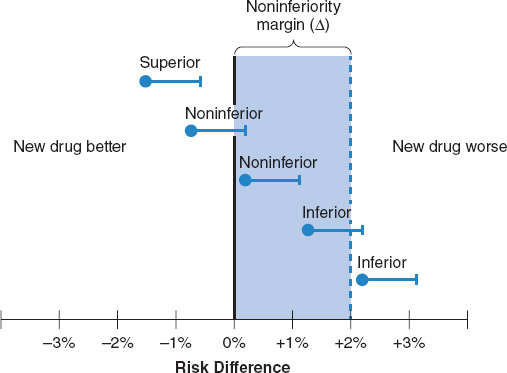
\includegraphics[width=11.661cm]{assets/ch12_figure02_original.png}};
\fill[white](230,0)rectangle(356,37);\node[font=\small,align=center]at(293,15){非劣效界值\\（$\Delta$）};
\fill[white](132,51)rectangle(205,72);\node[font=\small]at(169,62){优效};
\fill[white](176,102)rectangle(234,126);\fill[chTwelveBand](235,102)rectangle(282,126);\node[font=\small]at(220,115){非劣效};
\fill[chTwelveBand](236,152)rectangle(335,177);\node[font=\small]at(275,165){非劣效};
\fill[chTwelveBand](290,201)rectangle(350,224);\fill[white](351,201)rectangle(368,224);\node[font=\small]at(325,215){劣效};
\fill[white](352,251)rectangle(430,274);\node[font=\small]at(388,265){劣效};
\fill[white](10,135)rectangle(156,157);\node[font=\small]at(83,147){新药更好};
\fill[white](380,130)rectangle(512,165);\node[font=\small]at(448,147){新药更差};
\fill[white](150,353)rectangle(330,380);\node[font=\small]at(238,366){风险差};
\draw[dashed,dcrblue,line width=.8pt](350,55)--(350,319);
\end{tikzpicture}}
\providecommand{\chTwelveCrossover}{\begin{tikzpicture}[font=\footnotesize,>=Stealth]
\draw[dashed,dcrred](0,0)ellipse(1.75 and 2.4);\node[text=dcrred]at(0,2.65){可接触人群};\node[align=center]at(0,1.75){符合选择标准的样本};
\node[draw=dcrred,text width=23mm,align=center](b)at(0,0){测量基线预测变量\\及适当情况下的\\结局基线值};
\node[circle,draw](r)at(2.3,0){R};\draw[->](b)--(r);
\foreach \yy/\txt/\nm in {1.6/设盲干预/ctop,-1.6/设盲对照/cbottom}{\node[draw=dcrteal,text width=19mm,align=center](\nm)at(4.1,\yy){实施\txt};\draw[->,dcrteal](r)--(\nm);}
\node[draw=dcrgold,minimum height=43mm,align=center](m)at(5.8,0){测\\量\\结\\局};
\node[draw,minimum height=43mm,align=center](w)at(6.7,0){洗\\脱\\期};
\draw[->,dcrteal](ctop.east)--(5.55,1.6);\draw[->,dcrteal](cbottom.east)--(5.55,-1.6);
\node[draw=dcrteal,text width=19mm,align=center](a)at(8.6,1.6){实施设盲干预};\node[draw=dcrteal,text width=19mm,align=center](c)at(8.6,-1.6){实施设盲对照};
\draw[->,dashed,dcrteal](5.2,1.6)--(7.5,-1.6);\draw[->,dashed,dcrteal](5.2,-1.6)--(7.5,1.6);
\node[draw=dcrgold,minimum height=43mm,align=center](e)at(10.3,0){测\\量\\结\\局};\draw[->](a)--(e);\draw[->](c)--(e);
\foreach \x in {4,8.5}{\draw[->,dcrteal](\x+.5,1.2)to[bend left=25](\x+.8,.6);\node[text=dcrteal]at(\x,.45){失访};\draw[->,dcrteal](\x+.5,-2)to[bend left=25](\x+.8,-2.6);\node[text=dcrteal]at(\x,-2.7){失访};}
\end{tikzpicture}}
\providecommand{\chTwelveCluster}{\begin{tikzpicture}[x=.018cm,y=-.018cm]
\node[anchor=north west,inner sep=0]at(0,0){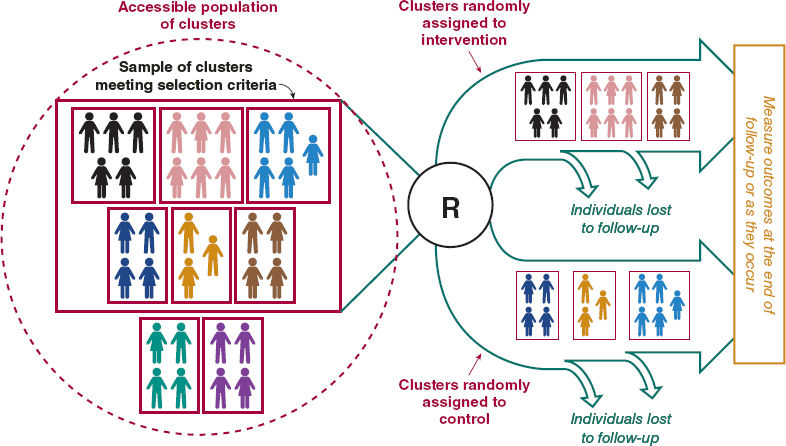
\includegraphics[width=14.148cm]{assets/ch12_figure04_original.png}};
\fill[white](108,0)rectangle(309,32);\node[font=\small]at(208,15){可接触人群中的群体};
\fill[white](91,55)rectangle(305,93);\node[font=\small,align=center]at(198,75){符合选择标准的群体样本};
\fill[white](395,0)rectangle(535,47);\node[font=\scriptsize,align=center,text=dcrred]at(465,22){随机分到\\干预的群体};
\fill[white](397,378)rectangle(535,427);\node[font=\scriptsize,align=center,text=dcrred]at(465,401){随机分到\\对照的群体};
\fill[white](550,198)rectangle(720,240);\node[font=\scriptsize,text=dcrteal]at(635,216){个体失访};
\fill[white](550,412)rectangle(720,451);\node[font=\scriptsize,text=dcrteal]at(635,430){个体失访};
\fill[white](737,48)rectangle(783,361);\node[font=\scriptsize,rotate=90,text=dcrgold]at(760,205){结局发生时或随访结束时测量结局};
\end{tikzpicture}}
\providecommand{\chTwelveStepped}{\begin{tikzpicture}[font=\footnotesize,x=.58cm,y=.42cm]
\foreach \row/\lab in {0/9,1/3,2/12,3/7,4/8,5/5,6/11,7/2,8/10,9/1,10/4,11/5}{
\node[anchor=east]at(0,-\row-.5){群\lab};
\pgfmathtruncatemacro{\start}{2*floor(\row/2)+3}
\foreach \col in {1,...,14}{\ifnum\col<\start\fill[white](\col-1,-\row)rectangle(\col,-\row-1);\else\fill[chTwelveBand](\col-1,-\row)rectangle(\col,-\row-1);\fi\draw[dcrblue,thin](\col-1,-\row)rectangle(\col,-\row-1);}}
\foreach \col in {1,...,14}{\node at(\col-.5,-12.6){\col};}
\foreach \col in {1,3,5,7,9,11,13}{\draw[dcrred](\col,-12)--(\col,0);}
\node at(7,-13.4){月};\draw[->,dcrblue](0,-14)--(0,-12.1);\node[anchor=east]at(0,-14.2){试验开始};\draw[->,dcrblue](14,-14)--(14,-12.1);\node[anchor=west]at(14,-14.2){试验结束};
\end{tikzpicture}}
\providecommand{\chTwelveBefore}{\begin{tikzpicture}[font=\small,>=Stealth]
\draw[dashed,dcrred](0,0)ellipse(2.3 and 2.4);\node[text=dcrred]at(0,2.7){可接触人群};\node[align=center]at(0,1.8){符合选择标准的参与者};
\node[draw=dcrred,text width=33mm,minimum height=27mm,align=center](b)at(0,0){\textcolor{dcrpurple}{测量基线预测变量}\\\textcolor{dcrgold}{测量结局基线值}};
\draw[->,thick,dcrteal](b)--node[above]{实施干预}(8,0);\node[draw=dcrgold,text=dcrgold,align=center]at(8.8,0){测量\\结局变量};
\foreach \x in {3.5,6}{\draw[->,dcrteal](\x,0)to[bend left=30](\x+.5,-1.6);}\node[text=dcrteal]at(5,-2){失访};
\draw[->,thick,dcrteal](1.8,-3)--(8.8,-3);\node[fill=white,text=dcrteal]at(5,-3){随访时间};\node[align=center]at(0,-3.2){研究起始\\（之前）};\node[align=center]at(9,-3.7){研究结束\\（之后）};
\end{tikzpicture}}
\providecommand{\chTwelveTimeSeries}{\begin{tikzpicture}[x=.026cm,y=-.026cm]
\node[anchor=north west,inner sep=0]at(0,0){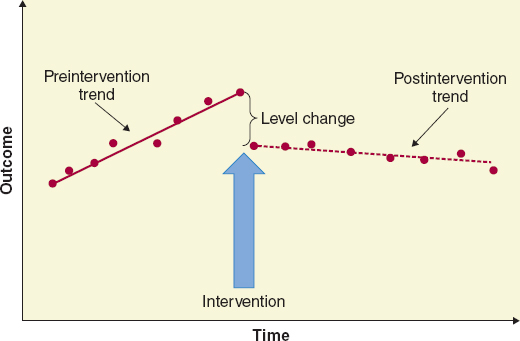
\includegraphics[width=13.52cm]{assets/ch12_figure07_original.png}};
\fill[chTwelveCream](40,64)rectangle(155,108);\node[font=\small,align=center]at(100,85){干预前趋势};
\fill[chTwelveCream](260,105)rectangle(380,135);\node[font=\small]at(320,120){水平变化};
\fill[chTwelveCream](390,65)rectangle(511,108);\node[font=\small]at(449,85){干预后趋势};
\fill[chTwelveCream](194,289)rectangle(293,316);\node[font=\small]at(244,302){干预};
\fill[white](0,122)rectangle(17,198);\node[font=\small,rotate=90]at(8,162){结局};
\fill[white](240,322)rectangle(315,345);\node[font=\small]at(277,333){时间};
\end{tikzpicture}}
\providecommand{\chTwelvePriors}{\begin{tikzpicture}[x=.0198cm,y=-.0198cm]
\node[anchor=north west,inner sep=0]at(0,0){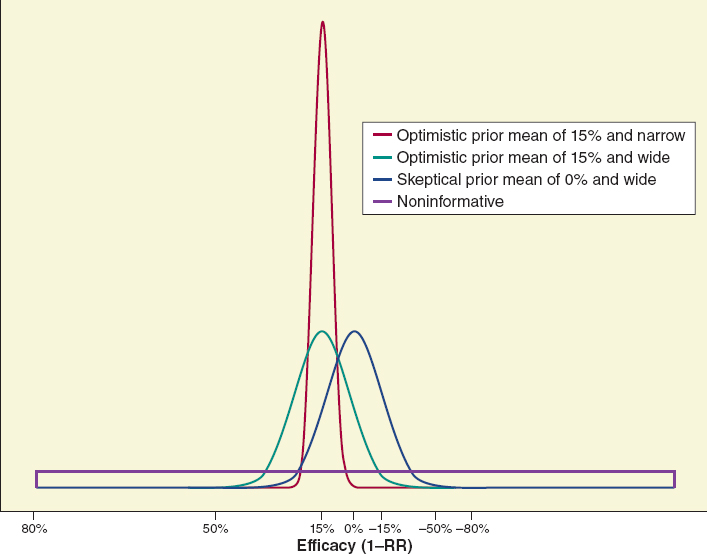
\includegraphics[width=13.9986cm]{assets/ch12_figurea01_original.png}};
\fill[white](396,124)rectangle(693,210);
\node[anchor=west,font=\scriptsize]at(398,136){乐观先验：均值15\%，分布窄};
\node[anchor=west,font=\scriptsize]at(398,158){乐观先验：均值15\%，分布宽};
\node[anchor=west,font=\scriptsize]at(398,180){怀疑先验：均值0\%，分布宽};
\node[anchor=west,font=\scriptsize]at(398,202){无信息先验};
\fill[white](292,536)rectangle(415,554);\node[font=\small]at(354,546){疗效（$1-\mathrm{RR}$）};
\end{tikzpicture}}

\sourcepage{378}
\begin{figure}[htbp]\centering\chTwelveFactorial
\caption*{\textbf{图12.1\quad 析因随机试验。}从适合接受各项干预（此例为药物）的可接触人群中选择参与者样本；测量基线预测变量，以及适当情况下的结局变量基线水平；考虑额外测量并保存标本，以备后续分析；将两种或更多活性药物及其安慰剂对照，随机分配（以R表示）到四组或更多组；随访参与者，尽量减少失访，评估对药物和安慰剂的依从性，并测量结局变量。分析结果时，先合并两个药物A组，与合并的安慰剂A组比较；再合并两个药物B组，与合并的安慰剂B组比较。}
\end{figure}
\sourcepage{379}
不过，析因设计的一个限制，是可能发生效应修饰。例如，维生素D3对心血管病风险的作用，可能因是否同时接受omega-3脂肪酸而异。如果确实如此，就必须分别在接受和未接受脂肪酸补充剂的参与者中，计算维生素D3的作用。这样，每次分析只纳入一半参与者，比较的统计效能便会降低。析因设计也可以专门用于研究效应修饰，但以此为目的的试验，实施和解释更复杂，需要更大的样本量。析因设计的其他限制是，同一目标人群必须同时适合两项干预，而且多种治疗可能妨碍招募与依从。

\subsection{活性对照：等效性与非劣效性试验}
在\term{活性对照试验}（active control trial）中，对照组也接受能影响所关注状况的干预。由于比较的是两种治疗，有时称为\term{比较效果试验}（comparative effectiveness trial）。当某疾病已有“标准照护”时，这可能是最佳设计。

有时，活性对照试验的目标是证明新治疗优于既有治疗，所用设计和方法与安慰剂对照试验相似。但通常，研究者希望证明新治疗在保持相近疗效的同时，比既有治疗更易使用、侵入性较低或更安全；如果“同类跟随”治疗没有这些优势，就很难说明为何值得开展试验。此时，\term{等效性试验}（equivalence trial）或\term{非劣效试验}（noninferiority trial）更合适。例如，多项研究已证明，对女性开展个体盆底肌训练，可以有效治疗尿失禁症状（3）。\sourcepage{380}随后一项比较个体训练与团体训练的试验发现，团体方法不劣于个体治疗（4），这可能使更多人有机会接受训练。

等效性和非劣效试验的统计方法，不同于旨在证明一种治疗优于另一种治疗的试验。在优效性试验中，标准分析用统计学显著性检验拒绝“两组没有差异”的零假设；而在旨在证明新治疗与标准治疗等效的试验中，目标则是发现两者没有差异。不过，要证明两种治疗之间连极小的差异都不存在，需要无限大的样本量。一个可行的解决方法，是根据新治疗相对于标准治疗的疗效差置信区间，设计样本量和分析。研究者预先指定两种治疗的疗效差，称为\term{非劣效界值}（noninferiority margin，delta或$\Delta$）：如果新治疗的疗效低了$\Delta$或更多，研究者便判定标准治疗更好（5、6）。相反，如果新治疗相对于既有治疗的疗效差置信区间不包含$\Delta$，就确立等效性或非劣效性（图12.2）。通常，研究者只希望证明新治疗不劣于标准治疗，因此采用单侧置信区间；其好处是允许使用较小样本量（第6章）。
\sourcepage{381}
\begin{figure}[htbp]\centering\chTwelveNoninferiority
\caption*{\textbf{图12.2\quad 非劣效试验的可能结果。}试验比较新药与华法林降低房颤患者卒中风险的作用，非劣效界值$\Delta$设为$+2\%$。图示华法林与新药卒中率之差的单侧95\%置信区间，分别说明优效、劣效和非劣效的结果。}
\end{figure}

确定非劣效界值既需要统计方面的考虑，也需要对新治疗潜在疗效与优势作临床判断（7）。一种设定$\Delta$的方法，是对既有治疗与安慰剂比较的既往试验进行荟萃分析，将零效应与治疗作用置信区间下限之间距离的一定比例，作为$\Delta$。不过，荟萃分析中的试验质量常不一致，因此，以入选标准、既有治疗剂量和结局测量均与当前试验相近、质量最佳的随机试验为依据，可能更好。设定$\Delta$时，应使研究者在综合考虑全部益处与危害之后，仍很有把握认为新治疗优于安慰剂（6、8）。非劣效试验通常比安慰剂对照试验规模更大，\sourcepage{382}因为新治疗与既有治疗之间可接受的差异，通常小于新治疗与安慰剂之间的预期差异。

非劣效并不一定意味着既有治疗与新治疗都有效：它们可能都无效，甚至都有害。为确保非劣效试验所评估的新治疗优于安慰剂，应有充分的既往研究资料支持既有治疗的疗效。这也意味着，非劣效试验的设计应尽量接近当初确立标准治疗疗效的试验，包括参与者选择标准、既有治疗的剂量与依从性、随访长度、失访等（6、8）。任何削弱标准治疗疗效的问题，例如纳入不太可能获益的参与者、不依从或失访，都会使新治疗更容易表现为非劣，因为标准治疗的作用已被削弱。实际疗效较差的新治疗，可能看起来不劣于标准治疗，而研究结果其实只反映了研究实施不佳。

\subsection{适应性设计}
经典临床试验依照研究期间不作改变的方案实施。不过，对于某些治疗和疾病，允许根据结果的中期分析修改试验方案的\term{适应性设计}（adaptive designs），可能更可取（9）。例如，一项非溃疡性消化不良新药的多剂量试验，最初计划在为期一年的招募期内，为安慰剂组及三个药物剂量组各招募50人，治疗12周。每组前10人完成4周治疗后，审查结果可能发现，只有最高剂量组出现了消化不良缓解的趋势。此时停止向两个较低剂量组分配参与者，仅继续随机比较最高剂量与安慰剂，可能更有效率。试验的其他方面也可根据中期结果改变，例如当中期结果提示效应量或结局发生率\sourcepage{383}与最初假定不同时，修改样本量或试验持续时间。

只有干预产生的结局能足够早地测量和分析，仍来得及改变设计时，适应性设计才可行。为防止偏倚，应在试验开始前明确如何改变设计的规则；中期分析和是否改变设计的考虑，应交由独立的数据监察委员会处理。中期分析增加了仅因偶然而发现有利结果的概率，统计分析必须考虑这一点。

\term{平台试验}（platform trials）及篮式试验、伞式试验等变体，是使用单一主方案，同时或依次评估多项干预的适应性试验（10）。平台试验通常评估干预组合、不同亚组的干预效果差异，或依次开展的多项干预。适应性平台可以宣布一项或多项干预或剂量具有优效性，同时继续评估其他干预；可以因缺乏疗效或有害而删除某项干预；还可以在试验期间加入新干预，继续使用同一主方案和试验设施。与一项试验只研究一项干预的传统策略相比，这类试验可能以更少的资源、更快地找到有效干预，也无须为每一项待研究干预另建试验设施。

例如，美国国立过敏与传染病研究所资助的适应性COVID-19治疗试验（Adaptive COVID-19 Treatment Trial，ACTT-1），就是依次研究严重急性呼吸综合征冠状病毒2（SARS-CoV-2）感染或COVID-19治疗的平台试验。首先研究的药物瑞德西韦，与安慰剂相比，缩短了恢复时间。该平台试验的设计允许在发现有效治疗后删除安慰剂组，同时继续将有益治疗与其他抗病毒药及免疫反应调节药比较（11）。

\term{贝叶斯试验}（Bayesian trials）在设计和分析时纳入其他资料，如关于相同或类似干预的既往研究，因此不同于通常称为频率学派试验的标准试验（附录12A）。\sourcepage{384}例如，一项频率学派试验将$\alpha$设为0.05，检验治疗是否使结局风险至少降低25\%。如果试验发现风险降低20\%，$P$值为0.09，该结果就不具有“统计学显著性”。相反，贝叶斯方法将治疗有效的先验概率用于试验分析与设计。例如，如果既往研究显示风险降低25\%，对相同结果进行贝叶斯分析，可能估计出：治疗使结局风险至少降低20\%的概率为99\%。

贝叶斯试验通常要求招募人数具有灵活性，不固定样本量或预算，也不采用根据多次查看资料而调整$P$值的停止规则。有些适应性试验使用既往研究结果规划下一项试验，也会采用贝叶斯方法。

\subsection{交叉设计}
在\term{交叉研究}（crossover study）中，一部分参与者随机先接受活性干预，再改为对照干预；另一部分先接受对照干预，再改为活性干预（图12.3）。这样既可作组间分析，即比较活性治疗组与对照组，也可作组内分析，即比较每位参与者接受干预和接受对照时的结果。其优点很大：每个人都作为自身对照，配对分析提高了统计效能，因此所需参与者少于平行组试验。

其缺点也很大：研究持续时间加倍；每个交叉期开始和结束时都要测量结局，因而增加费用；潜在的\term{残留效应}（carryover effects）还使分析和解释更复杂。残留效应是停止干预后仍然存在的影响，例如一个疗程的利尿药治疗结束数月后，血压仍未回到基线水平。为减少残留效应，研究者可以在两种治疗之间加入不接受治疗的\term{洗脱期}（washout period），\sourcepage{385}希望结局变量在开始下一项干预之前回到基线水平；不过，很难确定全部残留效应是否都已消除。一般而言，当研究参与者数量有限、结局对干预的反应迅速且可逆时，交叉研究是一个良好选择。
\begin{figure}[htbp]\centering\chTwelveCrossover
\caption*{\textbf{图12.3\quad 交叉试验。}从适合接受干预的可接触人群中选择参与者样本；测量基线预测变量，以及适当情况下的结局变量基线水平；随机分配（以R表示）设盲的干预与对照条件；随访参与者，尽量减少失访，评估对干预和对照条件的依从性，并测量结局变量；停止干预和对照，适当时设置洗脱期以减少残留效应；将原对照组改为接受干预，原干预组改为接受对照，继续随访后测量结局。}
\end{figure}

\sourcepage{386}
\subsection{等待名单设计}
若所研究的干预不能设盲，而且参与者认为新型非侵入性操作等干预比对照更理想，交叉设计的一种变体可能适用。此时，可能很难找到愿意随机进入对照组的合格参与者。一个很好的替代方法，是随机分配参与者在试验开始时接受干预，或进入等待名单对照组，在规定时间后接受干预。等待名单对照的另一种适用情况是：医院、社区、学校、政府等机构虽然只有有限的疗效依据，却已出于政治或公平考虑，决定让某群体的所有成员接受干预。此时，将开始干预的时间随机延后，可能是可以接受的。

\term{等待名单设计}（wait-list design）为立即干预组与等待名单对照组的随机比较提供了机会。此外，可以合并两个干预时期，即一组的立即干预期与另一组的延后干预期，以提高组内干预前后比较的统计效能。例如，有症状的子宫肌瘤女性可以随机接受子宫动脉栓塞等新治疗，或进入6个月后获提供子宫动脉栓塞的等待名单对照组。随后，既可以比较最初随机接受子宫动脉栓塞与最初进入等待名单者的肌瘤症状评分变化，也可以合并所有接受干预者的组内症状评分变化。

等待名单设计要求结局在足够短的时间内发生，以免等待时间过长。此外，在试验末期给对照组提供干预，会延长随访时间并增加试验费用。

\subsection{单例设计}
\sourcepage{387}
\term{单例设计}（N-of-1 designs，$N$表示样本量），也称单患者试验，类似于只纳入一人的交叉试验，通常旨在回答某位患者的疗效或不良作用等临床问题。最简单的单例试验先将患者随机分配到一段固定时间的设盲治疗，或安慰剂（也可以是另一种活性治疗），再交叉接受另一种干预，持续相同时间。也可以安排多次交叉，以提供更有力的结局资料。

例如，一位频繁发生偏头痛的患者与他的医师，认为加巴喷丁可能减少头痛频率，但并不确定，他们可以同意开展单例试验。试验可以包含数个时期，患者在每个时期随机接受加巴喷丁或安慰剂。患者在试验开始时及此后定期记录头痛频率。结局通常由患者根据最困扰自己的症状选择，并用简单的李克特量表（Likert scale）评分。在计划的试验终点，通常为2～5个交叉期之后，揭盲并评估资料。有时只需查看资料，就足以决定最佳治疗；也可以采用配对$t$检验或时间序列方法等统计方法。

群体试验回答的是一组参与者的临床问题，其中可能有人获益，有人不获益；与之相比，单例试验的优点在于可能回答某位具体患者的问题。不过，它最适合慢性或反复出现症状的疾病，要求结局能在治疗后迅速改变，停药后作用也迅速消退。与交叉试验相同，可以设置洗脱期，尽量减少治疗的残留效应，但洗脱所需时间往往不明确。患者必须理解试验要求，并愿意接受设盲治疗；若不设盲，结果可能并不比临床判断更好。单个临床医师通常难以独立开展单例试验，需要研究药房或“单例试验服务（N-of-1 Service）”的协助（12）。

\sourcepage{388}
\subsection{整群随机设计}
在\term{整群随机设计}（cluster randomized designs）中，研究者将自然形成的参与者群体或群随机分配到各项干预，而不是对个人进行随机分配（图12.4）。一项研究大学棒球队员的试验就是很好的例子：研究纳入120支大学棒球队，将其中一半球队随机分配到鼓励戒除嚼烟的干预组。结果发现，干预院校有35\%的队员戒除了嚼烟，对照院校的比例则为16\%（13）。
\begin{figure}[htbp]\centering\chTwelveCluster
\caption*{\textbf{图12.4\quad 整群随机试验。}从适合接受干预的可接触人群中抽取若干群；测量群内成员的基线预测变量，以及适当情况下的结局变量基线水平；将各群随机分配（以R表示）到设盲的干预或对照条件；随访参与者，尽量减少失访，并评估他们对干预或对照条件的依从性；测量结局变量。}
\end{figure}

\sourcepage{389}与逐人随机相比，将一项干预随机分配给若干群体可能更容易实施，成本效益也可能更好；这种方法也可能更适合回答人群公共卫生项目或医疗服务系统内质量改进干预的效果问题。有些干预，例如低脂饮食，可能很难只在一个家庭的一名成员中实施。如果对自然群体内的参与者逐人随机，接受干预的人很可能与分在对照组的家人、同事、队友或熟人讨论或分享干预。因此，对照组也可能接触干预，这种\term{沾染}（contamination）会降低观察到的干预疗效。电子决策支持或临床流程改变等质量改进措施，尤其难以在患者个人层面随机，因为同一名临床医师、同一家诊所或同一个临床单元，很可能同时照护被分到干预组和对照组的患者，从而发生干预沾染。

必须区分整群随机试验与按组实施干预的试验。例如，在瑜伽或太极研究中，参与者通常在个人层面随机分组，但可能通过集体训练课接受干预。同一瑜伽班或太极班的参与者，其干预效果可能存在聚集性，因此需要作统计调整。不过，随机分配仍在个人层面实施，所以这不是整群随机试验。

整群随机设计的随机单位是群，而不是个人。有效样本量小于参与者总人数，取决于各群内参与者干预效果的相关程度，其数值介于群数和参与者总人数之间（14）。一般而言，群数较多而每群人数较少，比群数较少而每群人数较多具有更高的统计效能（15）。

\sourcepage{390}整群随机试验的另一个潜在问题，是各干预组的基线特征可能不平衡。随机单位很多时，随机分配最有利于使特征得到平衡；整群随机则减少了随机单位的数量。例如，一项试验虽有数千名参与者，但他们只分布于四个地理区域，其中一个区域与另外三个很不相同，那么随机后的研究组之间就会不平衡。按群体规模、男性比例或合并症患病率等进行分层随机或匹配随机，可能有助于处理各群重要混杂因素不同的问题，但不能解决上述例子中的问题。

整群随机的其他缺点是，样本量估计和资料分析都比个体随机更复杂（9）。

\subsection{阶梯楔形设计}
\term{阶梯楔形试验}（stepped wedge trial）是整群随机设计的一种变体：一个群、一组群或单个参与者接受的随机分配，并不是决定其接受干预还是作为对照，而是决定其开始干预的顺序（16、17）。试验首先设一个收集基线资料的时期，此时所有群都不接受干预。随后，在试验期间预先规定的时间间隔（称为“台阶”），随机选择各群开始干预。一旦某群开始干预，就持续到试验结束；到试验结束时，所有群都已接受干预（图12.5）。由于每个群都经历对照和干预两种状态，既可作群间比较，也可作群内比较。同一时期中，随机处于干预和对照状态的群之间的比较，可以控制时间效应或队列效应；同一群内结局变化的比较，则能减少群间差异可能引入的混杂。这类试验的示意图呈“阶梯楔形”（图12.5），设计由此得名。
\sourcepage{391}
\begin{figure}[htbp]\centering\chTwelveStepped
\caption*{\textbf{图12.5\quad 阶梯楔形试验。}所有群（此处为12个）起初均处于对照状态（白色）。在固定时点（此处每隔2个月），随机选定若干群（此处为2个）开始干预（蓝色）。各群一旦开始干预，就持续到试验结束。该设计因图形的形状而称为“阶梯楔形”。译注：底本第6行和末行均标“群5”，未标群6；图中保留此重复编号。}
\end{figure}

阶梯楔形设计最常用于临床流程、公共卫生干预或质量改进研究。除了前述整群随机的优点，它还可能在政治或文化上更容易被接受，更可行，也更符合伦理。与等待名单设计相似，当医院、社区、学校或政府虽然只有有限的疗效依据，却已决定让某群体的所有成员接受干预时，阶梯楔形设计可能最为合适。此外，资源有限或实施安排复杂，可能使大型复杂干预无法在整个医疗系统同时开展，此时逐步推广可能最容易实施。例如，在Mesita Azul干预研究中，UC Berkeley的研究者与当地一家非营利组织合作，在南下加利福尼亚的24个乡村社区开展阶梯楔形试验，评估紫外线消毒饮水处理系统的效果。研究将这些社区划为六个群，按随机顺序引入干预；该干预降低了饮用水被大肠埃希菌污染的\sourcepage{392}家庭比例，但没有降低腹泻患病率（18）。

与所有整群随机试验一样，阶梯楔形试验的有效样本量取决于群内成员之间的相关性，介于群数与参与者总人数之间。因此，阶梯楔形试验所需的样本量可能远大于个体随机试验。这类试验通常规模大、组织复杂，需要与医疗系统或政府的领导者密切合作。在阶梯楔形试验中，对照状态的资料平均而言早于干预状态的资料收集。因此，医疗服务或资料收集随时间发生、与干预本身无关的变化，可能混杂研究结果。分析也较复杂，既要考虑整群设计，又要考虑结局的时间趋势。阶梯楔形试验所采用的干预，常被认为已有研究依据，目的是在通常照护的基础上提高质量。在这种情况下，尤其当结局可以用公开资料或常规医疗过程中收集的资料确定时，机构审查委员会（Institutional Review Board，IRB）可能豁免逐人取得知情同意的要求。

\section{非随机干预设计}
当伦理、政治、社会或实施条件使随机试验无法开展时，可以比较未经过随机分配的各组所接受的干预效果；这类试验常称为准实验或准随机设计。第10章已介绍其中一些设计，并称其为“机会性”设计，因为它们依赖某种机会，例如政策改变所创造的机会，估计某项变化对结局的作用。机会性设计属于观察性研究：研究者不设计或实施所研究的变化。与之相比，本章讨论的是非随机干预性研究设计，即研究者设计并实施干预，但不以随机方式分配干预。

\sourcepage{393}这类试验常用于评估政策、医疗实践改变，或已有研究依据的做法的实施效果。不过，非随机试验控制混杂变量的能力远不及随机试验。例如，试验若比较冠状动脉旁路移植手术与经皮血管成形术的效果，却允许临床医师决定哪些患者接受哪种操作，而不采用随机分配，那么被选中接受手术的患者，很可能与被选中接受血管成形术的患者不同。分析方法可以调整两组间已测量的基线因素差异，却不能解决未测量混杂的问题（见第10章）。将针对同一研究问题的随机研究与非随机研究结果相比，即使已对基线变量的差异作统计调整，非随机研究观察到的干预益处也常常更大（19）。

有时，参与者通过一种模仿随机分配的机制进入各研究组。例如，将医院病历号为偶数的所有参与者分配到治疗组。这类设计可能便于实施，但伪随机分配并不能保证各组基线可比，而且可以预知的分组结果，可能使研究者或研究工作人员操纵新参与者的入组顺序或入选资格。例如，如果知道某位候选者将进入活性治疗组，就可能优先纳入比一般人更健康的候选者。

选择非随机设计，有时是因为误以为允许参与者或临床医师自行选择干预，会比随机分配更符合伦理。我们认为，研究只有在有合理可能正确回答研究问题时才符合伦理，而非随机研究比随机设计更不容易得到正确结果。此外，任何试验的伦理基础，都是尚不确定干预究竟有益还是有害。这种不确定性称为\term{临床均势}（equipoise）；它意味着无法根据已有研究资料选择干预，\sourcepage{394}也构成采用随机分配的理由。

\subsection{非随机组内设计}
\subsubsection{前后试验}
\term{前后试验设计}（before-after或pre-post trial designs）比较实施干预之前与之后的结局（图12.6），相当于没有对照组的单臂干预试验。前后设计应用广泛，尤其常见于政策、流程和指南改变的效果研究，以及临床质量改进研究。其主要优点是，可能避开随机设计所面临的伦理顾虑，而且通常费用低、实施简单（20）。
\begin{figure}[htbp]\centering\chTwelveBefore
\caption*{\textbf{图12.6\quad 前后试验。}从适合接受干预的可接触人群中选择参与者样本；测量基线预测变量和结局变量；对整个样本实施干预；随访样本，尽量减少失访并评估干预依从性；在干预期结束后测量结局。}
\end{figure}

\sourcepage{395}如果在干预前后测量的是同一批参与者，那么每个人都作为自身对照。年龄、族裔和遗传因素等个人特征，不只是像随机组间研究那样得到平衡，而是不再作为混杂变量产生影响。例如，为研究培训项目的效果，可以比较高年级医学生在干预前后准确判读心电图（electrocardiogram，ECG）的能力。不过，许多前后试验是在不同的人群中测量结局。若引入一项干预以降低医院获得性艰难梭菌感染的发生率，干预前后的发生率很可能来自不同患者。此时，比较结果仍容易受到年龄、疾病严重程度等常见混杂变量差异的影响。

时间效应、均数回归和成熟效应，也会大幅削弱前后设计中的因果推断。疾病发生率或临床照护随时间、季节发生的变化，不论有无干预都可能影响结局。疾病报告方式、病例定义以及许多与干预同时发生的其他变化，都可能使前后研究的结局随时间改善。例如，一项研究若引入新的手部消毒剂以减少医院获得性感染，那么人员配备变化、工作人员培训、个人防护装备使用增加或季节性暴发，都可能解释感染率的变化。

干预前后的变化也可能来自\term{均数回归}（regression to the mean），即测量值回归或移回其均数的倾向。自然生物变异及测量精密度不足，使多数测量值随时间波动。若研究纳入切点设在这种波动范围的高端或低端，后续测量值便很可能更接近总体均数。例如，某人的收缩压在\sourcepage{396}130～160 mmHg之间随机波动，而试验要求血压大于150 mmHg才能入组，那么无论干预有何作用，入组后的测量值都可能仅因均数回归而低于入组切点。如果实施某项干预，是因为它所要预防的结局最近发生频率升高，也会出现同样的问题。例如，医院获得性感染率的偶然波动，可能促使感染控制人员在观察到高感染率时引入干预。随后感染率因均数回归而下降，便可能让干预显得有效。

即使没有干预，人们、工作人员和临床医师也往往会随着时间学习并有所改善，这称为\term{成熟效应}（maturation effect）。例如，在一项旨在延缓阿尔茨海默病患者认知衰退的无对照前后试验中，参与者可能仅因越来越熟悉认知功能测试，而自然地提高测试表现。最后，许多前后研究持续时间不够长，无法判断干预效果能否维持。

在干预前多次测量结局，以确认结局没有明显变化，有时可以减少时间变化、均数回归和成熟效应的影响。例如，在一项用β受体阻滞剂减少偏头痛发作频率的前后试验中，可以先用数个月的资料，计算一组患者干预前的平均每周头痛次数。增强因果推断的另一种方法，是加入预先规定的证伪检验：证明干预会影响所关注的结局，却不会影响那些本来不应因干预而改变的其他结局。例如，在用新型抗逆转录病毒药作暴露前预防、以防止人类免疫缺陷病毒感染的前后研究中，研究者还可以测量其他性传播疾病（sexually transmitted diseases，STDs）的发生率；抗逆转录病毒药不应影响这些疾病。如果开始治疗后，HIV与其他性传播疾病的发生率出现了相近幅度的下降，就提示观察到的药物益处可能源于危险性行为减少。

\sourcepage{397}
\subsubsection{中断时间序列}
\term{中断时间序列设计}（interrupted time series designs）与前后设计相似，但要求在干预前多次测量，以估计结局的趋势或斜率，这个趋势随后被干预“中断”。干预后的多次测量，则用于确定引入干预后，结局的水平或趋势是否改变；其中水平变化，是第一个干预后时点的观察值与按原趋势预测的结局水平之差（图12.7）。该设计假定，如果没有干预，干预前的趋势会继续保持不变（21）。
\begin{figure}[htbp]\centering\chTwelveTimeSeries
\caption*{\textbf{图12.7\quad 中断时间序列。}干预前多次测量结局，以确定干预前的结局趋势或斜率（实线）；实施干预后再次多次测量，以识别干预之后结局水平是否立即改变（花括号），并确定干预后的结局趋势（虚线）。干预由此“中断”了结局测量序列。}
\end{figure}

中断时间序列研究必须清楚地区分干预前和干预后的时期，最适合干预后能较快发生变化的结局。按照惯例，干预前后各至少需要\sourcepage{398}三次测量，才能计算结局趋势；测量次数更多，统计效能也更高。不过，这在实践中可能难以做到。

与前后研究相似，在随机试验无法开展时，中断时间序列也常用于评估政策、流程或实践改变的影响。其优点是能够考虑干预前已有的结局趋势。不过，季节变化、资料收集或分类方法改变、疾病暴发，以及同时发生的其他政策或实践改变，都容易使中断时间序列结果受到混杂。加入一个与干预组相似的对照组，可以处理其中一部分问题，下一节将作讨论。

\subsection{含非随机对照的设计}
前后研究与中断时间序列研究都可以加入非随机对照组。\term{受控前后研究}（controlled before-after study），有时也称有非等效对照组的前后研究，是在干预前后同期测量两组参与者的结局。对照应选自与干预组相似、但未接受干预的人群、地区或诊所。主要结局是干预组与对照组结局变化量之差，通常称为\term{双重差分}分析。如果两组都经历相同的季节、政策和流程变化，那么结局的组间差异由干预引起，就更为可信。如果所需测量不多，而且两组资料都可以从相同来源（如电子健康记录）获得，这种设计通常容易实施。类似地，受控中断时间序列设计加入非随机对照组，以两组结局水平变化或趋势变化之差作为结局。

均数回归仍是受控前后研究的一个主要问题，尤其当干预组是因疾病暴发或疾病水平较高而被选中，而对照组没有出现相同情况时。上述两种设计都没有采用随机分配，\sourcepage{399}因而干预组与对照组可能存在差异，例如季节、流程或资料收集的变化不同，这些差异可能混杂干预的作用。\footnote{译注：底本此小节标题再次写作“Nonrandomized Within-Group Designs”，但内容讨论加入非随机对照，且小结第10项称组间设计；此处按段落所述译为“含非随机对照的设计”。}

\section{小结}
在适当情况下，可以对经典的个体水平随机、盲法、平行组试验作如下变通：
\begin{enumerate}
\item 析因随机试验设计通过将参与者随机分配到多项干预，在一项试验中回答两个或更多独立的研究问题。不过，一项干预对另一项干预产生的效应修饰可能降低试验效能，而且研究人群必须适合其中的每一项干预。
\item 非劣效试验有时用于比较新干预与已有治疗，以确定两者疗效之差是否不超过一个预先规定、具有临床重要性的数值。当已有标准照护时，非劣效试验可能合适，但所需样本量通常大于新干预与安慰剂比较的试验。
\item 适应性设计允许根据结果的中期分析修改试验方案，对某些干预而言可能是一种高效率的研究方法。平台试验通过一个适应性主方案评估多项干预，与传统试验设计相比，可能以更少的资源、更快地找到有效干预。
\item 在交叉设计中，一部分参与者随机先接受活性干预，另一部分先接受对照干预；随后，两组“交叉”接受另一种干预。这样，每名参与者都作为自身对照；配对分析提高了统计效能，因此所需参与者少于平行组试验。
\sourcepage{400}
\item 在等待名单试验中，参与者随机分为试验开始即接受干预的一组，以及经过规定时间后接受干预的等待名单对照组。如果干预很有吸引力，这种设计能大幅提高招募的可行性；当所有合格参与者最终都将接受干预时，它也使随机比较成为可能。
\item 单例设计是只纳入一人的交叉试验，目的是回答某位患者的疗效或不良作用等临床问题。
\item 整群随机试验将参与者的群体或群随机分配到干预，而不是对个人随机分配。与逐人随机相比，将干预随机分配给群体可能更容易实施，成本效益也可能更好。
\item 阶梯楔形试验将个人、单个群或若干群随机分配到开始干预的先后顺序；到试验结束时，所有参与者都已接受干预。当政治、文化或公平方面的考虑要求群体所有成员都接受干预时，阶梯楔形设计最为合适。
\item 当伦理、政治、社会或实施条件使随机试验无法开展时，可以采用非随机组内设计，比较未经随机分配的群体中的干预效果。这些设计包括：
\begin{enumerate}
\item 个体前后设计在实施干预前后测量结局的水平或频率（如体重），以确定干预后结局是否改变；人群前后设计则测量干预前后某个人群中的结局发生频率。
\item 中断时间序列设计要求在干预前后多次测量，以估计引入干预时结局水平的变化，或干预后结局趋势（斜率）的变化。与前后研究相比，中断时间序列设计的优点是能够考虑干预前已有的结局趋势。
\end{enumerate}
\item 非随机组间设计：前后研究和中断时间序列研究可以加入非随机对照组。\sourcepage{401}受控前后研究在干预前后同期测量两组参与者的结局，主要结局是双重差分，即干预组与对照组结局随时间变化量之差。加入对照组可以考虑季节、政策和流程变化，从而增强因果推断。
\end{enumerate}
\begin{references}
\item Manson JE, Cook NR, Lee I-M, et al. Vitamin D supplements and prevention of cancer and cardiovascular disease. N Engl J Med. 2019;380:33-44.
\item Manson JE, Cook NR, Lee I-M, et al. Marine n−3 fatty acids and prevention of cardiovascular disease and cancer. N Engl J Med. 2019;380:23-32.
\item Dumoulin C, Cacciari LP, Hay-Smith EJC. Pelvic floor muscle training versus no treatment, or inactive control treatments, for urinary incontinence in women. Cochrane Database Syst Rev. 2018;10(10):CD005654.
\item Dumoulin C, Morin M, Danieli C, et al., for the Urinary Incontinence and Aging Study Group. Group-based vs individual pelvic floor muscle training to treat urinary incontinence in older women: a randomized clinical trial. JAMA Intern Med. 2020;180(10):1284-1293.
\item Piaggio G, Elbourne DR, Altman DG, et al. Reporting of non-inferiority and equivalence randomized trials. An extension of the CONSORT Statement. JAMA. 2006;295:1152-1160.
\item Piaggio G, Elbourne DR, Pocock SJ, et al. Reporting of non-inferiority and equivalence randomized trials. An extension of the CONSORT 2010 statement. JAMA. 2012;308:2594-2604.
\item D’Agostino RB Sr., Massaro JM, Sullivan LM, et al. Non-inferiority trials: design concepts and issues—the encounters of academic consultants in statistics. Statist Med. 2003;22:169-186.
\item Kaul S, Diamond GA. Good enough: a primer on the analysis and interpretation of non-inferiority trials. Ann Intern Med. 2006;145:62-69.
\item Chang M, Chow S, Pong A. Adaptive design in clinical research: issues, opportunities, and recommendations. J Biopharm Stat. 2006;16:299-309.
\item Berry SM, Connor JT, Lewis RJ. The Platform Trial: an efficient strategy for evaluating multiple treatments. JAMA. 2015;313:1619-1620.
\item Beigle JH, Tomashek KM, Dodd LE, et al., for the ACTT-1 Study Group Members. Remdesivir for the treatment of Covid-19—final report. N Engl J Med. 2020;383:1813-1826.
\item Guyatt G, Sackett D, Taylor DW, et al. Determining optimal therapy— randomized trials in individual patients. N Engl J Med. 1986:314:889-892.
\item Walsh M, Hilton J, Masouredis C, et al. Smokeless tobacco cessation intervention for college athletes: results after 1 year. Am J Public Health. 1999;89:228-234.
\item Donner A, Birkett N, Buck C, et al. Randomization by cluster: sample size requirements and analysis. Am J Epidemiol. 1981;114:906-914.
\item Cook AJ, Delong E, Murray DM, et al. Statistical lessons learned for designing cluster randomized pragmatic clinical trials from the NIH health care systems collaboratory biostatistics and design core. Clin Trials. 2016;13:504-512.
\item Hemming K, Haines TP, Chilton PJ, et al. The stepped wedge cluster randomised trial: rationale, design, analysis, and reporting. BMJ. 2015;350:h391.
\item Ellenberg SS. The stepped-wedge clinical trial. Evaluation by rolling deployment. JAMA. 2018;319:607-608.
\item Gruber JS, Reygadas F, Arnold BF, Ray I, Nelson K, Colford JM. A stepped wedge, cluster-randomized trial of a household UV-disinfection and safe storage drinking water intervention in rural Baja California Sur, Mexico. Am J Trop Med Hyg. 2013;89(2):238-245.
\item Chalmers T, Celano P, Sacks H, et al. Bias in treatment assignment in controlled clinical trials. N Engl J Med. 1983;309:1358-1361.
\item Sedgwick P. Before and after study designs. BMJ. 2014;349:g5074.
\item Bernal JL, Cummings S, Gasparrini A. Interrupted time series regression for the evaluation of public health interventions: a tutorial. Int J Epidemiol. 2017;46:348-355.
\end{references}

\sourcepage{402}
\chapterappendix{12A}{贝叶斯临床试验}
\sourcepage{403}
多数临床试验，例如研究双膦酸盐能否降低帕金森病患者髋部骨折风险的试验，旨在给定统计学显著性水平（$\alpha$）下，检验治疗是否具有某个指定的作用，如使结局风险降低20\%。研究的样本量估计、招募与随访计划以及预算，都据此安排。研究完成后，研究者比较干预组与对照组的髋部骨折风险，计算检验统计量的$P$值，判断结果是否达到统计学显著性。如果安排中期分析，可以将$\alpha$除以中期分析次数，或以其他方式分配。这种研究设计与资料分析的\term{频率学派}（frequentist）方法，依据的是：如果目标人群中的零假设为真，样本中出现所观察到的研究结果或更极端结果的频率会有多高（见第5章）。它不纳入关于双膦酸盐对髋部骨折作用的任何既有信息。

相反，对于同一个研究问题，\term{贝叶斯方法}（Bayesian approach）（1—3）会考虑此前许多研究的结果，这些研究已表明，双膦酸盐能降低无帕金森病者的髋部骨折风险（表12A.1）。该方法首先为帕金森病患者的每一种疗效水平指定\term{先验概率}。举一个简化的例子：双膦酸盐无益甚至有害的先验概率可能为0.2，髋部骨折风险降低不超过20\%的概率为0.3，降低20\%或更多的概率为0.5；这些比例之和必须为1.0。随着研究中髋部骨折的发生，将观察资料与这些先验概率结合，便得到新的可能性，称为\term{后验概率}（posterior probabilities）。临床试验的贝叶斯方法，类似于临床医师将疾病的检验前概率与诊断检验结果结合，以确定疾病检验后概率的做法（4）。

\sourcepage{404}
\begin{longtable}{L{27mm}L{61mm}L{61mm}}
\caption*{\textbf{表12A.1\quad 临床试验的频率学派与贝叶斯方法}}\\\toprule
概念&频率学派方法&贝叶斯方法\\\midrule\endfirsthead
\toprule 概念&频率学派方法&贝叶斯方法\\\midrule\endhead
试验结果&用点估计和置信区间表示治疗作用&治疗作用的后验分布、后验均数或中位数，以及可信区间\\
对既有研究资料的考虑&即使使用，也只是主观地用于解释$P$值&分析必须指定疗效的先验概率分布；完全没有既有资料时，通常采用平坦先验或怀疑先验（见正文）\\
统计学显著性或充分疗效依据&零假设的$P$值小于预先规定的阈值，通常为0.05&疗效的后验概率较高；申请新治疗的监管批准时，要求可能更严格\\
关于疗效的临床专家意见的作用&无&用于设定先验概率分布，通常涉及判断既有研究结果在多大程度上适用于当前试验\\
主观决定&将$P$值解释为存在治疗作用的可能性；规定样本量估计所需的参数；规定资料监察方式；选择分析模型&选择先验概率分布；选择分析模型\\
样本量&根据效应量、$\alpha$和$\beta$预先规定；效应量通常是尽可能合理的猜测&可以不预先规定；持续纳入参与者，直至有效、有害或无效的概率达到某一水平。有时也通过估计获得充分资料所需的预定样本量来设定\\
预算&固定样本量使预算可以固定&完全序贯的贝叶斯设计需要灵活的预算\\
资料监察与停止规则&在指定时点分析资料；基于$P$值的停止规则要对中期分析次数作调整&结果可不断更新，无须因反复分析而作惩罚性调整；新的后验概率取代原来的后验概率\\\bottomrule
\end{longtable}
\sourcepage{405}
治疗有效的先验概率不是一个数，甚至也不是前例中的几个数，而是表示为\term{先验分布}（prior distribution）。它通常是一条正态分布的钟形曲线，将疗效作为连续变量，估计不同疗效出现的可能性（图12A.1）。当我们对治疗作用知道得很多时，先验分布较窄；既有资料有限时，分布较宽。理想情况下，先验分布应依据此前针对类似研究问题的高质量研究结果；但有时必须依赖专家意见与主观判断。
\sourcepage{406}
\begin{figure}[htbp]\centering\chTwelvePriors
\caption*{\textbf{图12A.1\quad 先验分布示例。}横轴表示治疗的疗效，定义为$1-\mathrm{RR}$，其中RR为治疗相对于对照的风险比；纵轴表示该疗效的先验概率。红线为较窄的先验分布，以15\%的疗效为中心；绿线为较宽的先验分布，同样以15\%为中心；蓝线为以0\%疗效为中心的怀疑先验；紫线为平坦的无信息先验，也以0\%为中心。每条曲线下的面积均为1.0。}
\end{figure}

如何确定先验分布呢？例如，一项新治疗只是对既有药物略作修改，而数项实施良好的试验已发现，该既有药物可将所关注结局的风险降低约15\%。此时，新治疗很可能有相近效果，可以据此采用位于有效一侧的乐观先验分布，例如获益范围为7.5\%～22.5\%。另一方面，如果此前类似药物的研究有限，例如只研究过对生物标志物的作用，那么\sourcepage{407}采用以零为中心、认为治疗带来巨大益处或危害的可能性都很小的怀疑先验分布，就比较合适。先验分布通常呈钟形，但无信息先验可以是平坦的，即在所有合理的获益或危害水平上均匀分布，以表示缺乏信息。

从既有研究结果得到的先验分布，常常还要与怀疑先验或无信息先验混合，从而加以修正。混合比例取决于专家判断：既有研究适用于当前临床情境的概率有多大。这样便生成一个新的先验分布。

分析资料时，贝叶斯试验不检验试验结果是否具有统计学显著性，而是将结果与先验分布结合，生成\term{后验分布}（posterior distribution），表示治疗作用可能落入的范围；通常用\term{可信区间}（credible interval）或\term{最高后验密度区间}（highest posterior density interval）概括。例如，假定所选先验分布有效，治疗作用落在90\%可信区间内的概率就是0.9。也可以将结果表示为某个治疗作用的概率，例如治疗使结局风险至少降低30\%的概率为0.94；这一表述同样以所选先验分布为前提。

贝叶斯方法可能得出与频率学派不同的结论。例如，Brophy（5）重新分析了一项试验，该试验将左主干冠状动脉疾病患者随机分配到经皮冠状动脉介入治疗（percutaneous coronary intervention，PCI）或冠状动脉旁路移植术（coronary artery bypass graft，CABG）。研究发现，PCI患者的主要结局，即5年内死亡、心肌梗死和卒中，明显多于CABG患者，但风险增加的95\%置信区间（$-0.9\%$～6.5\%）包含零。因此，采用频率学派方法时，研究结论是PCI与CABG的结局没有显著差异，这一结论能给读者传达的信息很有限。相反，贝叶斯方法纳入此前研究类似问题的试验结果后，估计PCI增加试验终点风险的概率为0.96。

\sourcepage{408}
贝叶斯试验的设计也在若干方面不同于经典随机试验。有时，可以估计获得充分资料、形成“足够窄”的后验分布所需的预期参与者人数，以此估计样本量，但不必预先固定。相反，可以采用序贯方法，随着结局资料不断收集，更新治疗有效或有害的概率。由于贝叶斯方法不依赖$P$值与$\alpha$，因此无须对多次查看资料作调整（6）。当该概率超过预先设定的有效、有害或徒劳阈值时，可以停止招募；徒劳意味着研究结果不大可能回答研究问题。当然，贝叶斯试验的研究者必须指定疗效的先验分布，规定如何决定是否修改该分布，例如是否与怀疑先验混合，还要规定研究期间是否更新这些决定，以及如何更新。

没有固定样本量的设计，有时称为“完全序贯”设计。由于研究开始时可能尚不知道样本量和随访时间，因此需要灵活的资助安排。资助者不能只拨出一笔固定预算，而必须接受研究可能比希望的时间更长、费用更多；当然，研究也可能比预期更早结束。

总的来说，贝叶斯试验在设计和分析时纳入关于干预疗效的既有资料。当既往资料足以帮助确定先验分布时，贝叶斯方法可能合适。如果观察结果与先验预期一致，贝叶斯试验有可能需要更小的样本量。此外，将研究结果表示为治疗疗效的一系列概率，可能比单个$P$值或置信区间提供更多信息。不过，贝叶斯方法依赖对先验分布的主观判断，其中包括既有资料在多大程度上适用于目标人群和所研究的治疗。它还要求预算具有灵活性，而美国国立卫生研究院（National Institutes of Health，NIH）等传统资助来源可能无法提供这种安排。
\sourcepage{409}
\begin{references}
\item Harrell FE, Jr. Introduction to Bayes for Evaluating Treatments. http://hbiostat.org/doc/bayes/course.html
\item Diamond GA, Kaul S. Prior convictions: Bayesian approaches to the analysis and interpretation of clinical megatrials. J Am Coll Cardiol. 2004;43(11):1929-1939.
\item Berry DA. Bayesian clinical trials. Nat Rev Drug Discov. 2006;5:27-36.
\item Browner WS, Newman TB. Are all significant P values created equal? The analogy between diagnostic tests and clinical research. JAMA. 1987;257:2459-2463.
\item Brophy JM. Bayesian interpretation of the EXCEL trial and other randomized clinical trials of left main coronary artery revascularization. JAMA Intern Med. 2020;180:986-992.
\item Gelman A, Hill J, Yajima M. Why we (usually) don’t have to worry about multiple comparisons. J Res Educ Effective. 2012;5:189-211.
\end{references}


\chapterappendix{12B}{第12章习题：其他干预性研究设计}
\sourcepage{410}
\begin{enumerate}
\item 非那雄胺（finasteride）是一种5α还原酶抑制剂，也是少数获得美国食品药品监督管理局（Food and Drug Administration，FDA）批准、用于治疗男性型脱发的药物之一。每日使用时，它对促进头发再生有中等程度的疗效，但停药6个月后作用即消失。另一类药物——他汀类——已被发现能通过与非那雄胺不同的生物学通路，增加啮齿类动物的毛发生长。假设一家初创公司想收集资料，证明一种新型外用他汀类药物HairStat治疗男性型脱发的疗效。针对以下每一种试验方法，至少列出一个优点和一个缺点。
\begin{enumerate}
\item 将男性型脱发者随机分配到HairStat或安慰剂组，两组均不提供非那雄胺。
\item 开展HairStat与非那雄胺的随机试验，比较两种治疗的疗效。
\item 将男性随机分配到HairStat或安慰剂组，但只招募此前使用非那雄胺未见获益，或不能耐受非那雄胺的人。
\item 采用析因试验设计，将男性随机分配到四组：（1）非那雄胺与HairStat联合；（2）非那雄胺与HairStat安慰剂；（3）非那雄胺安慰剂与HairStat；（4）双安慰剂。
\item 开展交叉试验，将男性随机分配到先用非那雄胺、3个月后改用HairStat，或按相反顺序用药的两组。
\end{enumerate}
\item 你在一家设有多个办公地点的大公司工作，公司希望减少员工肥胖，并促进健康饮食习惯。一位顾问建议实施多成分饮食干预，包括发放营养宣传册、在工作场所食堂开展营养宣传、在公共区域张贴教育海报，以及按照轮班时间安排饮食意识工作坊。你想评估这项干预能否促进超重或肥胖员工减重。以下实施和评估方法各有哪些潜在优点或缺点？
\begin{enumerate}
\item 在全公司范围内，将员工个人随机分配到饮食支持干预或无干预组，并评估6个月内每个人的体重变化。
\item 在公司的所有办公地点同时实施干预，持续6个月，比较员工干预前后的体重变化。\sourcepage{411}
\item 开展阶梯楔形试验，在6个月内按随机顺序，依次将饮食干预引入公司的所有办公地点。
\item 开展整群随机试验，将公司的各办公地点随机分配到实施饮食支持干预或不实施干预的两组。
\end{enumerate}
\end{enumerate}

\endgroup
